\chapter[Conclusion \&~Open Problems]{Conclusion \fancyand~Open Problems}
\label{ch:conclu-automatic}
\renewcommand\thefigure{\thechapter.\arabic{figure}}

\begin{chapterpresentation}
	\begin{abstract}
		This chapter concludes \Cref{part:automatic} of this thesis.
		We recall some open problems mentioned previously,
		and highlight a new research direction relating the
		structural properties of a language-theoretic framework
		with its expressiveness.
	\end{abstract}
	% \medskip
	% \begin{acknowledgements}
	% \end{acknowledgements}
	\par\bigskip\bigskip
	\chaptertoc
\end{chapterpresentation}

\section{Separating Automatic Relations by Recognizable Ones}

\begin{marginfigure}
	\centering
	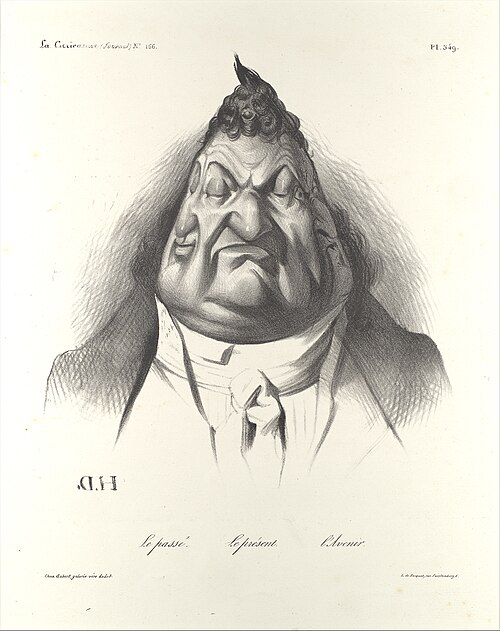
\includegraphics[width=\linewidth]{fig/PastPresentFuture.jpg}
	\caption{\href{https://www.metmuseum.org/art/collection/search/365043}{\emph{Le passé – Le présent – L'Avenir}}, by Honoré Daumier.}
\end{marginfigure}
The problem introduced in \Cref{ch:preliminaries-automatic-structures}
remains open.

\openProblemAutRecSeparability*

In \Cref{ch:dichotomy-theorem}, we proved this problem to be equivalent
to "finite regular colourability of automatic graphs" (\Cref{thm:reg-colourability-equiv-separability}),
and showed that when the number of colours is fixed, the problem is undecidable
(\Cref{thm:k-reg-col-undec}).
In fact, we showed that most problems of this form are undecidable
(\Cref{thm:dichotomy-theorem-automatic-structures}).
In turn, it implies that this separability problem becomes
undecidable when the "separator@@rel" is restricted to be
a union of $k$ products of "regular languages" for some fixed $k\geq 2$.
However, as explained in \Cref{sec:dichotomy-discussion}, some gaps remain to be able to use
our techniques to prove the undecidability of the "$\AUT$/$\REC$-separability problem".

On the other hand, we introduced in \Cref{ch:algebra} an algebraic approach for
"automatic relations", hoping to prove the decidability of this problem.
Algebraic language theory is a powerful tool to prove the decidability of separation
over finite words \cite{PlaceZeitoun2016SeparatingRegularLanguages},
but also in more complex settings such as countable ordinal words \cite{ColcombetGoolMorvan2022FOSeparation}.

Alas, using the theory we developped to tackle \Cref{opb:AUT-REC-separability}
seems non-trivial. The main obstacle being that, while
"recognizable relations" have some desirable closure properties,
they do not form a "pseudovariety of automatic relations".
% \todo{addref-discuss-algebra}.%
% \footnote{Explain why we couldn't know this \emph{a priori}.}

However, should \Cref{opb:AUT-REC-separability} problem be decidable, the question of
the decidability of its generalization to larger class of relations would be
a natural next step.

\begin{openproblem}
	Are the "$\DRAT$/$\REC$-separability@@pb" and
	"$\RAT$/$\REC$-sepa\-ra\-bility problems" decidable?
\end{openproblem}

In \cite[\S~1]{BarceloFigueiraMorvan2023SeparatingAutomatic},
we incorrectly stated that ``As for definability\footnote{Definability is the same
as the "membership problem".}, the "$\REC$-separability problem" for "rational relations" is in general undecidable'', which is unfounded as we do not currently know if it is true.
Indeed, as mentioned in \Cref{ch:preliminaries-automatic-structures},
the "$\RAT$/$\REC$-membership problem" is undecidable, by
\cite[\S~III, Theorem~8.4]{Berstel1979Transductions}.
Moreover, in general, "membership problems" reduced to "separability problems":
a relation $\+R$ belongs to a class $\+V$ if, and only if, $\+R$ and $\negrel \+R$
are "$\+V$-separable@@rel". However, for this argument to work, the larger class of relation
needs to be effectively closed under complement.
This is not the case of "rational relations", see \Cref{sec:prelim-rational-relations}.

For "deterministic rational relations", while they are effectively
closed under complement, the "$\DRAT$/$\REC$-membership problem"
is decidable---see \Cref{sec:prelim-automatic-drat}!

\section{Colouring Problems on Automatic Graphs}

Let us quickly recall some of the conjectures that have been discussed in \Cref{sec:dichotomy-discussion}.
The first one is about finding an equivalent characterization in the "dichotomy theorem
for automatic structures" (\Cref{thm:dichotomy-theorem-automatic-structures}).

\conjInvarianceGraphIsomorphisms*

In other words, this conjecture could be rephrased as follows: ``a problem
of the form $\HomRegAut{\?B}$ is decidable if, and only if, its output
only depends on the "structure represented" by the "automatic presentation",
and not on the "presentation@@auto" itself''!
Going back to our original question,
while we do not know if "finite regular colourability of automatic graphs"
is decidable, it is natural to study variations of this problem, as well as
sufficient or necessary conditions to ensure colourability or non-colourability.
Unfortunately, these problems are also non-trivial.

\conjFiniteColourabilityUndecidable*

\conjUnboundedCliques*

\section{An Algebraic Approach Beyond Automatic Relations}

The algebraic theory developed in \Cref{ch:algebra} can be generalized,
by replacing the constraint of ``being "well-formed"'' with an arbitrary
"regular language" $\Omega$. This would result in the notion
of \AP""$\Omega$-path algebras""---with "$\WellFormed$-path algebras" corresponding
to our "synchronous algebras".

While there is no hope to get a version of the
"lifting theorem" (\Cref{thm:lifting-theorem-monoids}) for every $\Omega$---see \Cref{rk:no-algo-lifting}---, we believe it holds for "fully-preordered languages".
See \Cref{sec:algebra-discussion} for more details.

Interestingly, we believe this question to be related to Figueira \& Libkin's
"$T$-controlled relations", presented in
\Cref{sec:preliminaries-automatic-structures-relations-restricted-head-movements}.
Each language $T$, specifying the head movements that are allowed,
gives rise to a language $\Omega_T$, such that relations recognized
by finite "$\Omega_T$-path algebras" exactly correspond to 
the "$T$-controlled relations".
\opbControlledRelations
We conjecture that, one way of tackling this problem would be to study properties of
the category of "$\Omega_T$-path algebras".

\conjAdjunctionControlledRelations*

\begin{marginfigure}
	\centering
	\includegraphics[width=\linewidth]{fig/Sieste.jpg}
	\caption{\href{https://commons.wikimedia.org/wiki/File:Henri_Manguin,_1905,_La_Sieste_(Le_repos,_Jeanne),_oil_on_canvas,_88.9_x_116.84_cm,_Villa_Flora,_Winterthur.jpg}{\emph{La Sieste}}, by Henri Manguin.}
\end{marginfigure}
Hopefully, the latter condition could maybe be massaged to get decidability.
Finally, \Cref{sec:theorem-projection-monad-adjunction} explains how the notion
of "monad adjunction" could provide a way of automatically projecting---or lifting,
depending on the point of view---an algebraic characterization from a universe to another.

\projectingAlgebraicCharacterization*